\documentclass[12pt]{article}

% Solutions toggle
\newif\ifsolutions
\solutionsfalse
%% \solutionstrue

% ASSIGNMENT NUMBER
\newcommand{\hwnumber}{2}
\newcommand{\booksection}{}
\newcommand{\duedate}{}
% -------------

%%% Packages
\usepackage[margin=1in, footskip=24pt, headheight=24pt]{geometry}
\usepackage{amsmath, amssymb, amsthm, graphicx}
\usepackage{mathtools}
\DeclarePairedDelimiter\ceil{\lceil}{\rceil}
\DeclarePairedDelimiter\floor{\lfloor}{\rfloor}
\usepackage[colorlinks, urlcolor=blue]{hyperref}
\usepackage{color}
\usepackage{comment}
\usepackage{enumerate}
\usepackage{lastpage}
\usepackage{multirow, multicol}
\usepackage{tikz}
\usetikzlibrary{matrix,decorations.text,decorations.pathmorphing,decorations.markings,arrows,calc,shapes.geometric,patterns,shadows,intersections,decorations.markings,decorations.pathreplacing,decorations.pathreplacing,backgrounds,angles,quotes}
\usepackage{pgfplots}
\pgfplotsset{compat=1.16}

\usepackage{fancyhdr}

\pagestyle{fancy}
%% \renewcommand{\familydefault}{\sfdefault}

\newcommand{\R}{\mathbb{R}}
\newcommand{\ddx}{\frac{d}{dx}}

\global\long\def\V#1{\boldsymbol{#1}} %vector
\global\long\def\M#1{\boldsymbol{#1}} %matrix

\global\long\def\D#1{\Delta#1} %\D{t} for time step size
\global\long\def\d#1{\delta#1} %\d{t} for small increment

\global\long\def\norm#1{\left\Vert #1\right\Vert }
\global\long\def\abs#1{\left|#1\right|}

\global\long\def\grad{\M{\nabla}}
\global\long\def\av#1{\left\langle #1\right\rangle }

% HEADER MACROS
\newcommand{\term}{Spring 2022 \& 2023}
\newcommand{\coursename}{Intro Math Modeling}
\newcommand{\coursenumber}{MATH-UA 251}
\newcommand{\course}{\coursename \ (\coursenumber)}

\fancyhead[RO]{\term}
\fancyhead[LO]{\course}
% -------------

%%% Theorem Styles
\theoremstyle{definition}
\newtheorem{ex}{Exercise}

%%%%%%%%%%%%%%%%%%%%%%%% Solutions %%%%%%%%%%%%%%%%%%%%%%%%%%%%%
% \begin{solution} and \begin{answerspace} must be at the beginning of the line.
% Doesn't work inside the \myversions command. Use if statements instead.
% No underscores in comment names

\ifsolutions
\newenvironment{solution}{\color{blue}}{} \excludecomment{answerspace} \newenvironment{notes}{\color{red} \noindent Grading Notes:}{}
\else
\excludecomment{notes} \excludecomment{solution} \includecomment{answerspace} 
\fi
%%%%%%%%%%%%%%%%%%%% End Solutions %%%%%%%%%%%%%%%%%%%%%%%e}


\begin{document}
% HEADER
\begin{center}
%% \ifsolutions
%%   \textbf{\Large Homework \hwnumber\ - \booksection\ (Solutions)}\\
%% \else
%%   \textbf{\Large Homework \hwnumber\ - \booksection}\\
%% \fi
\ifsolutions
  \textbf{\Large Homework \hwnumber\ (Solutions)}\\
\else
  \textbf{\Large Homework \hwnumber}\\
\fi
\vspace{12pt}
Due date: someday, sometime! \duedate

Submit on NYU Brightspace.
\end{center}

%% \noindent Please give complete, well-written solutions to the following exercise. Provide sufficient justification and explanation for a classmate who has not worked on the exercise to understand your solution.


% -------------------

\vspace{0.5cm}\noindent\textbf{Spherical Coordinates:} The spherical coordinate system uses a distance $r$ from the origin along with two angles $\theta$ and $\phi$ to uniquely locate a point in space. An elemental volume in spherical coordinates is illustrated below:

% https://tex.stackexchange.com/questions/429159/how-to-draw-a-differential-volume-element-with-tikz
\begin{center}
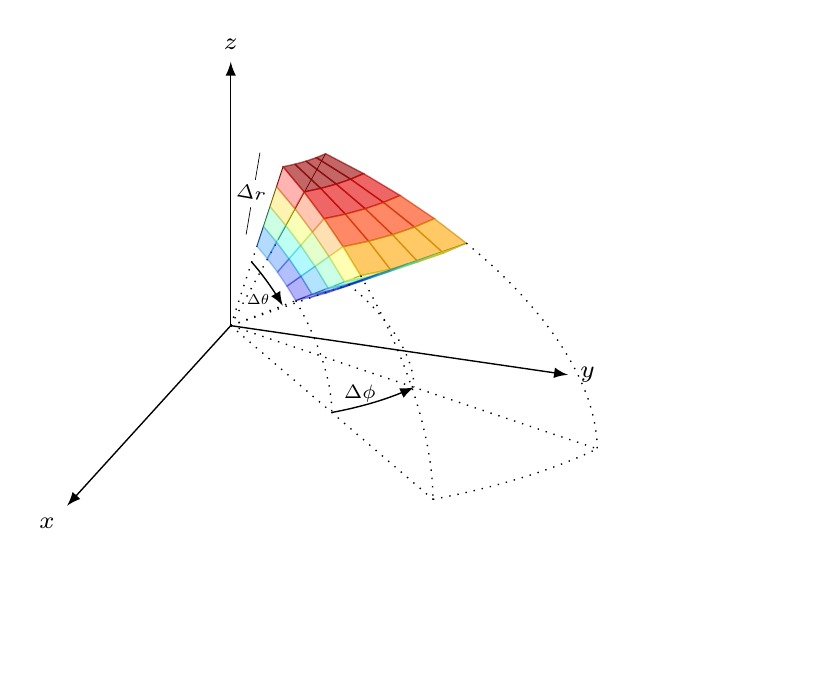
\begin{tikzpicture}[scale=1.25]
  \begin{axis}[axis line style={draw=none}, 
      view={110}{36},
      grid=major,
      xmin=0.5,xmax=2.5,
      ymin=0.5,ymax=2.5,
      zmin=0,zmax=2.5,
      enlargelimits=upper,
      xtick=\empty,
      ytick=\empty,
      ztick=\empty,
      clip=false
    ]

    \pgfmathsetmacro\tO{45};
    \pgfmathsetmacro\dt{25};
    \pgfmathsetmacro\phiO{15};
    \pgfmathsetmacro\dphi{25};

    \pgfmathsetmacro\phil{\phiO};
    \pgfmathsetmacro\phih{\phiO+\dphi};
    \pgfmathsetmacro\thetal{\tO}
    \pgfmathsetmacro\thetah{\tO+\dt}

    \addplot3[black,domain=0:1,samples=2,samples y=0,  dotted]
    ({x*cos(\thetal)*sin(\phil)},{x*sin(\thetal)*sin(\phil)},{x*cos(\phil)});

    \addplot3[black,domain=0:1,samples=2,samples y=0,  dotted]
    ({x*cos(\thetal)*sin(\phih)},{x*sin(\thetal)*sin(\phih)},{x*cos(\phih)});

    \addplot3[black,domain=0:1,samples=2,samples y=0,  dotted]
    ({x*cos(\thetah)*sin(\phil)},{x*sin(\thetah)*sin(\phil)},{x*cos(\phil)});

    \addplot3[black,domain=0:1,samples=2,samples y=0,  dotted]
    ({x*cos(\thetah)*sin(\phih)},{x*sin(\thetah)*sin(\phih)},{x*cos(\phih)});

    \addplot3[black,domain=1:2,samples=2,samples y=0, line width=0.2 ]
    ({x*cos(\thetal)*sin(\phil)},{x*sin(\thetal)*sin(\phil)},{x*cos(\phil)})
    node[left, yshift=-3mm, scale=0.8, xshift=-1mm, rotate=-10] {\scriptsize $\Delta r$};

    \pgfmathsetmacro\phim{\phiO-\dphi/4};
    \addplot3[black,domain=1:1.3,samples=2,samples y=0, line width=0.2 ]
    ({x*cos(\thetal)*sin(\phim)},{x*sin(\thetal)*sin(\phim)},{x*cos(\phim)});
    \addplot3[black,domain=1.6:1.9,samples=2,samples y=0, line width=0.2 ]
    ({x*cos(\thetal)*sin(\phim)},{x*sin(\thetal)*sin(\phim)},{x*cos(\phim)});

    \addplot3[black,domain=1:2,samples=2,samples y=0, line width=0.1, dashed ]
    ({x*cos(\thetal)*sin(\phih)},{x*sin(\thetal)*sin(\phih)},{x*cos(\phih)});

    \addplot3[black,domain=1:2,samples=2,samples y=0  , line width=0.2]
    ({x*cos(\thetah)*sin(\phil)},{x*sin(\thetah)*sin(\phil)},{x*cos(\phil)});

    \addplot3[black,domain=1:2,samples=2,samples y=0  , line width=0.2]
    ({x*cos(\thetah)*sin(\phih)},{x*sin(\thetah)*sin(\phih)},{x*cos(\phih)});
    
    \addplot3[surf,domain=\thetal:\thetah,y domain =\phil:\phih, samples=5, samples y=5, opacity=0.6, colormap/jet  ]
    ({2*cos(x)*sin(y)},{2*sin(x)*sin(y)},{2*cos(y});

    \addplot3[surf,domain=1:2,y domain =\phil:\phih, samples=5, samples y=5, opacity=0.3, colormap/jet  ]
    ({x*cos(\thetal)*sin(y)},{x*sin(\thetal)*sin(y)},{x*cos(y});

    \addplot3[surf,domain=1:2,y domain =\thetal:\thetah, samples=5, samples y=5, opacity=0.3, colormap/jet  ]
    ({x*cos(y)*sin(\phih)},{x*sin(y)*sin(\phih)},{x*cos(\phih});

    \coordinate (Z) at (0, 0, {cos(\phil)});
    \pgfmathsetmacro\s{cos(\thetal)*sin(\phil)};
    \pgfmathsetmacro\t{sin(\thetal)*sin(\phil)};

    \addplot3[black,domain=\phih:90,samples=20,samples y=0, dotted]
    ({2*cos(\thetah)*sin(x)},{2*sin(\thetah)*sin(x)},{2*cos(x)});

    \addplot3[black,domain=\phih:90,samples=20,samples y=0, dotted]
    ({2*cos(\thetal)*sin(x)},{2*sin(\thetal)*sin(x)},{2*cos(x)});

    \addplot3[black,domain=\phih:90,samples=20,samples y=0, dotted]
    ({cos(\thetah)*sin(x)},{sin(\thetah)*sin(x)},{cos(x)});

    \addplot3[black,domain=\phih:90,samples=20,samples y=0, dotted]
    ({cos(\thetal)*sin(x)},{sin(\thetal)*sin(x)},{cos(x)});

    \addplot3[black,domain=\thetal:\thetah,samples=20,samples y=0, dotted]
    ({2*cos(x)*sin(90)},{2*sin(x)*sin(90)},{2*cos(90)});

    \coordinate (O) at (0,0,0);
    \coordinate (A1) at ({2*cos(\thetal)}, {2*sin(\thetal)}, 0);
    \draw[dotted] (O)--(A1);
    \coordinate (A2) at ({2*cos(\thetah)}, {2*sin(\thetah)}, 0);
    \draw[dotted] (O)--(A2);

    \addplot3[black,domain=\thetal:\thetah,samples=20,samples y=0, -latex]
    ({1.0*cos(x)*sin(90)},{1.0*sin(x)*sin(90)},{1.0*cos(90)}) node[above, xshift=-5.5mm, yshift=-2.5mm, scale=0.8] {\scriptsize $\Delta \phi$};

    \addplot3[black,domain=\phil:\phih,samples=20,samples y=0  , -latex]
    ({0.8*cos(\thetal)*sin(x)},{0.8*sin(\thetal)*sin(x)},{0.8*cos(x)}) node[above, xshift=-2.5mm, yshift=-0.65mm, scale=0.6] {\scriptsize $\Delta \theta$};

    {\draw[color=black,-latex] (0,0,0) -- (2.0,0,0) node[anchor=north east]{\scriptsize $x$};}% x-axis
    {\draw[color=black,-latex] (0,0,0) -- (0,1.5,0) node[anchor=west]{\scriptsize $y$};}% y-axis
    {\draw[color=black,-latex] (0,0,0) -- (0,0,2.5) node[anchor=south]{\scriptsize $z$};}% z-axis

  \end{axis}
\end{tikzpicture}
\end{center}
The radial distance $r$ is measured from the origin; the angle $\phi\in[0,2\pi)$ varies in the $xy$ plane and is zero on the $x$ axis; the angle $\theta\in[0,\pi]$ measures the deviation from the $z$ axis. The projected radius onto the $xy$ plane is $r\sin(\theta)$. The radii of curvature for angles $\theta$ and $\phi$ are $r$ and $r\sin(\theta)$, respectively. Therefore, we have the following formula for the volume of the element, $V$, and area in different directions (treating the elemental volume as a rectangular box for small $\Delta r,\Delta\theta,\Delta\phi$):
  \begin{align*}
    V&=(\Delta r)\cdot(r\Delta\theta)\cdot(r\sin(\theta)\Delta\phi)=r^2\sin(\theta)\Delta r\Delta\theta\Delta\phi,\\
    A_r&=(r\Delta\theta)\cdot(r\sin(\theta)\Delta\phi)=r^2\sin(\theta)\Delta\theta\Delta\phi,\\
    A_{\theta}&=(\Delta r)\cdot(r\sin(\theta)\Delta\phi)=r\sin(\theta)\Delta r\Delta\phi,\\
    A_{\phi}&=(\Delta r)\cdot(r\Delta\theta)=r\Delta r\Delta\theta.
  \end{align*}
  Here, $A_{r},\;A_{\theta},\;A_{\phi}$ denote the area in the $r,\;\theta,\;\phi$ directions.

\newpage
\begin{ex}
    
[50 pts] The mass flux (mass per unit area per unit time) can be expressed as
$$\rho \mathbf{u}=\rho u_r\hat{e}_r+\rho u_{\theta}\hat{e}_{\theta}+\rho u_{\phi}\hat{e}_{\phi},$$
where $\rho$ is density of the material and $\mathbf{u}$ is the vector of velocity with scalar components $u_r,\;u_{\theta},\;u_{\phi}$ in $r,\;\theta,\;\phi$ directions, respectively.

\textcolor{purple}{Write a shell balance for the elemental volume to derive the differential form of the continuity equation in spherical coordinates. Next, simplify your answer for constant $\rho$.}
		
\begin{solution}
  We write the shell balance as
  \begin{align*}
    &\frac{\partial}{\partial t}(\rho r^2\sin(\theta)\Delta r\Delta\theta\Delta\phi)=\\
    &+(\rho u_r r^2\sin(\theta)\Delta\theta\Delta\phi)_{r}-(\rho u_r r^2\sin(\theta)\Delta\theta\Delta\phi)_{r+\Delta r}\\
    &+(\rho u_{\theta} r\sin(\theta)\Delta r\Delta\phi)_{\theta}-(\rho u_{\theta} r\sin(\theta)\Delta r\Delta\phi)_{\theta+\Delta\theta}\\
    &+(\rho u_{\phi} r\Delta r\Delta\theta)_{\phi}-(\rho u_{\phi} r\Delta r\Delta\theta)_{\phi+\Delta\phi}.
  \end{align*}
  Divide both sides by $\Delta r\Delta\theta\Delta\phi$ and let $\Delta r,\Delta\theta,\Delta\phi\to 0$:
  \begin{align*}
    \frac{\partial}{\partial t}(\rho r^2\sin(\theta))=&\lim_{\Delta r\to 0}{\frac{(\rho u_r r^2\sin(\theta))_{r}-(\rho u_r r^2\sin(\theta))_{r+\Delta r}}{\Delta r}}\\
    +&\lim_{\Delta\theta\to 0}{\frac{(\rho u_{\theta} r\sin(\theta))_{\theta}-(\rho u_{\theta} r\sin(\theta))_{\theta+\Delta\theta}}{\Delta\theta}}\\
    +&\lim_{\Delta\phi\to 0}{\frac{(\rho u_{\phi} r)_{\phi}-(\rho u_{\phi} r)_{\phi+\Delta\phi}}{\Delta\phi}}.\\
    \Rightarrow r^2\sin(\theta)\frac{\partial\rho}{\partial t}=&-\frac{\partial}{\partial r}(\rho u_r r^2\sin(\theta))-\frac{\partial}{\partial\theta}(\rho u_{\theta} r\sin(\theta))-\frac{\partial}{\partial\phi}(\rho u_{\phi} r).
  \end{align*}
  Finally, divide both sides by $r^2\sin(\theta)$ to get\textcolor{teal}{
  \begin{equation*}
    \frac{\partial\rho}{\partial t}+\frac{1}{r^2}\frac{\partial}{\partial r}(\rho u_r r^2)+\frac{1}{r\sin(\theta)}\frac{\partial}{\partial\theta}(\rho u_{\theta}\sin(\theta))+\frac{1}{r\sin(\theta)}\frac{\partial}{\partial\phi}(\rho u_{\phi})=0.
  \end{equation*}}%
  If density is constant (i.e, not a function of time or location), the continuity equation simplifies to\textcolor{teal}{
  \begin{equation*}
    \frac{1}{r^2}\frac{\partial}{\partial r}(u_r r^2)+\frac{1}{r\sin(\theta)}\frac{\partial}{\partial\theta}(u_{\theta}\sin(\theta))+\frac{1}{r\sin(\theta)}\frac{\partial}{\partial\phi}(u_{\phi})=0.
  \end{equation*}}
  
\end{solution}

\end{ex}

\begin{ex}
    
[50 pts] The heat flux (thermal energy per unit area per unit time) can be expressed as
$$\rho\mathbf{u}C_p T-k\mathbf{\nabla} T,$$
where the new parameters $C_p,\;k,\;T$ are the specific heat capacity, thermal conductivity, and temperature, respectively, and the gradient operator in spherical coordinates is
$$\mathbf{\nabla} T=\frac{\partial T}{\partial r}\hat{e}_r+\frac{1}{r}\frac{\partial T}{\partial\theta}\hat{e}_{\theta}+\frac{1}{r\sin(\theta)}\frac{\partial T}{\partial\phi}\hat{e}_{\phi}.$$

\textcolor{purple}{Write a shell balance (with a heat source $s$) for the elemental volume to derive the differential form of the heat equation in spherical coordinates. Next, simplify your answer for constant $\rho,\;C_p,\;k$.}
		
\begin{solution}
  The total heat flux in each direction, $\gamma_{r,\theta,\phi}$, can be expressed as
  \begin{align*}
    \gamma_r&=\rho u_rC_pT-k\frac{\partial T}{\partial r},\\
    \gamma_{\theta}&=\rho u_{\theta}C_pT-\frac{k}{r}\frac{\partial T}{\partial \theta},\\
    \gamma_{\phi}&=\rho u_{\phi}C_pT-\frac{k}{r\sin(\theta)}\frac{\partial T}{\partial \phi}.
  \end{align*}
  We then write the energy balance as
  \begin{align*}
    &\frac{\partial}{\partial t}(\rho r^2\sin(\theta)\Delta r\Delta\theta\Delta\phi C_p T)=sr^2\sin(\theta)\Delta r\Delta\theta\Delta\phi\\
    &+(\gamma_r r^2\sin(\theta)\Delta\theta\Delta\phi)_{r}-(\gamma_r r^2\sin(\theta)\Delta\theta\Delta\phi)_{r+\Delta r}\\
    &+(\gamma_{\theta} r\sin(\theta)\Delta r\Delta\phi)_{\theta}-(\gamma_{\theta} r\sin(\theta)\Delta r\Delta\phi)_{\theta+\Delta\theta}\\
    &+(\gamma_{\phi} r\Delta r\Delta\theta)_{\phi}-(\gamma_{\phi} r\Delta r\Delta\theta)_{\phi+\Delta\phi}.
  \end{align*}
  Following the same procedure as in Exercise 1, divide both sides by $r^2\sin(\theta)\Delta r\Delta\theta\Delta\phi$, let $\Delta r,\Delta\theta,\Delta\phi\to 0$, and use the definition of derivative to get:
  \begin{equation*}
    \frac{\partial(\rho C_p T)}{\partial t}+\frac{1}{r^2}\frac{\partial}{\partial r}(\gamma_r r^2)+\frac{1}{r\sin(\theta)}\frac{\partial}{\partial\theta}(\gamma_{\theta}\sin(\theta))+\frac{1}{r\sin(\theta)}\frac{\partial}{\partial\phi}(\gamma_{\phi})=s.
  \end{equation*}
  Now substituting for $\gamma_{r,\theta,\phi}$ yields
  \begin{align*}
    &\frac{\partial(\rho C_p T)}{\partial t}+\frac{1}{r^2}\frac{\partial}{\partial r}\left(r^2\left[\rho u_rC_pT-k\frac{\partial T}{\partial r}\right]\right)\\
    +&\frac{1}{r\sin(\theta)}\frac{\partial}{\partial\theta}\left(\sin(\theta)\left[\rho u_{\theta}C_pT-\frac{k}{r}\frac{\partial T}{\partial \theta}\right]\right)\\
    +&\frac{1}{r\sin(\theta)}\frac{\partial}{\partial\phi}\left(\rho u_{\phi}C_pT-\frac{k}{r\sin(\theta)}\frac{\partial T}{\partial \phi}\right)=s.
  \end{align*}
  Upon some rearrangements we obtain the heat balance equation as\textcolor{teal}{
  \begin{align*}
    &\frac{\partial(\rho C_p T)}{\partial t}+\frac{1}{r^2}\frac{\partial}{\partial r}\left(r^2\rho u_rC_pT\right)+\frac{1}{r\sin(\theta)}\frac{\partial}{\partial\theta}\left(\sin(\theta)\rho u_{\theta}C_pT\right)+\frac{1}{r\sin(\theta)}\frac{\partial}{\partial\phi}\left(\rho u_{\phi}C_pT\right)\\
    &=\frac{1}{r^2}\frac{\partial}{\partial r}\left(r^2k\frac{\partial T}{\partial r}\right)+\frac{1}{r^2\sin(\theta)}\frac{\partial}{\partial\theta}\left(k\sin(\theta)\frac{\partial T}{\partial \theta}\right)+\frac{1}{r^2\sin^2(\theta)}\frac{\partial}{\partial\phi}\left(k\frac{\partial T}{\partial \phi}\right)+s.
  \end{align*}}%
  For constant $\rho,\;C_p,\;k$, the equation simplifies to
  \begin{align*}
    &\frac{\partial T}{\partial t}+\frac{1}{r^2}\frac{\partial}{\partial r}\left(r^2u_rT\right)+\frac{1}{r\sin(\theta)}\frac{\partial}{\partial\theta}\left(\sin(\theta)u_{\theta}T\right)+\frac{1}{r\sin(\theta)}\frac{\partial}{\partial\phi}\left(u_{\phi}T\right)\\
    &=\frac{k}{\rho C_p}\left[\frac{1}{r^2}\frac{\partial}{\partial r}\left(r^2\frac{\partial T}{\partial r}\right)+\frac{1}{r^2\sin(\theta)}\frac{\partial}{\partial\theta}\left(\sin(\theta)\frac{\partial T}{\partial \theta}\right)+\frac{1}{r^2\sin^2(\theta)}\frac{\partial^2 T}{{\partial \phi}^2}\right]+\frac{s}{\rho C_p}.
  \end{align*}
  One can further simplify the left hand side by using the product rule, and then the continuity equation for constant density:
  \begin{align*}
    &\frac{\partial T}{\partial t}+\frac{1}{r^2}\left[r^2u_r\frac{\partial T}{\partial r}+T\frac{\partial r^2u_r}{\partial r}\right]+\frac{1}{r\sin(\theta)}\left[\sin(\theta)u_{\theta}\frac{\partial T}{\partial \theta}+T\frac{\partial \sin(\theta)u_{\theta}}{\partial \theta}\right]+\frac{1}{r\sin(\theta)}\left[u_{\phi}\frac{\partial T}{\partial \phi}+T\frac{\partial u_{\phi}}{\partial \phi}\right]\\
    =&\frac{\partial T}{\partial t}+T\left[\frac{1}{r^2}\frac{\partial}{\partial r}(r^2 u_r)+\frac{1}{r\sin(\theta)}\frac{\partial}{\partial\theta}(u_{\theta}\sin(\theta))+\frac{1}{r\sin(\theta)}\frac{\partial}{\partial\phi}(u_{\phi})\right]+u_r\frac{\partial T}{\partial r}+\frac{u_{\theta}}{r}\frac{\partial T}{\partial\theta}+\frac{u_{\phi}}{r\sin(\theta)}\frac{\partial T}{\partial\phi}\\
    =&\frac{\partial T}{\partial t}+T\left[0\right]+u_r\frac{\partial T}{\partial r}+\frac{u_{\theta}}{r}\frac{\partial T}{\partial\theta}+\frac{u_{\phi}}{r\sin(\theta)}\frac{\partial T}{\partial\phi}.
  \end{align*}
  Therefore,\textcolor{teal}{
  \begin{align*}
    &\frac{\partial T}{\partial t}+u_r\frac{\partial T}{\partial r}+\frac{u_{\theta}}{r}\frac{\partial T}{\partial\theta}+\frac{u_{\phi}}{r\sin(\theta)}\frac{\partial T}{\partial\phi}\\
    &=\frac{k}{\rho C_p}\left[\frac{1}{r^2}\frac{\partial}{\partial r}\left(r^2\frac{\partial T}{\partial r}\right)+\frac{1}{r^2\sin(\theta)}\frac{\partial}{\partial\theta}\left(\sin(\theta)\frac{\partial T}{\partial \theta}\right)+\frac{1}{r^2\sin^2(\theta)}\frac{\partial^2 T}{{\partial \phi}^2}\right]+\frac{s}{\rho C_p}.
  \end{align*}}
  
\end{solution}

\end{ex}

\end{document}
